\section{CHARACTER CLASSIFICATION}
\label{sec:class}

\subsection{Initial thoughts}
% After having looked at the dataset, did you have any initial idea about what kind of model that might work well?  Explain your reasoning.
OCR involves interpreting images and inferring characters. With this in mind, Artificial Neural Networks (ANN's) became a natural choice the task. ANN's excel at performing object recognition tasks. Their popularity have risen dramatically in recent years, partially due to the high accuracy they achieve in tasks that involve computer vision. Especially effective for problems like OCR is the Convolutional Neural Networks (CNN's). The intuition of using a CNN aroused from its very nature: they preserve the spatial relationship between pixels in an image, and use this to extract surprisingly abstract features in their classification process. The networks are also very modular as a large variety of layers can be applied.

To compare with the CNN, we wanted a \textit{simpler} and a less complex method that would provide adequate classification accuracy. We chose to use an SVM, which is widely recognized in classification problems, so there should not be too large of a gap between the models when classifying the letters. A CNN is a non-linear classifier because of its use of non-linear activation functions, whereas an SVM is a linear classifier because it uses kernels to project features onto a hyperplane where it is possible to separate the classes linearly. 

\subsection{Choice of classifiers}
% Give a description of the two models you elected to use. The description must include a brief explanation on how they work. Why did you select these models?
\subsubsection{SVM}
The Scikit implementation of a multiclass SVM uses a "one-vs-one" approach and might look cumbersome when it comes to computational time \cite{sklearn_api}. However, compared to something like k-NN, which must evaluate the dataset every time, we will have a trained model that can be applied easily. The main reason for choosing an SVM was because we wanted to compare it with the CNN algorithm. Before implementation, we hypothesized that the CNN would outperform the SVM, which would not necessarily be true for OCR.

\begin{figure}[H]
    \centering
    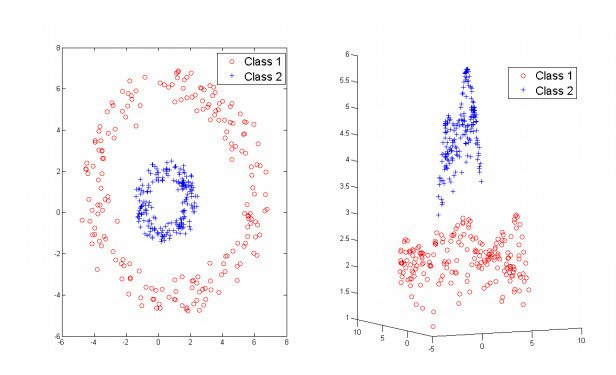
\includegraphics[width=0.45\textwidth]{pictures/SVM.png}
    \caption{The SVM finds a hyperplane (r.h.s.) that makes the classes linearly seperable.}
    \label{fig:SVM}
\end{figure}

SVM is a supervised machine learning algorithm that can be employed for both classification and regression purposes. Basically, SVM finds a hyperplane that divides the dataset (Figure \ref{fig:SVM}). Support vectors are the points nearest to the hyperplane. The hyperplane may be altered if any support vectors are removed from the dataset.

SVM uses different kernels to find the hyperplane. Although the model has auto-tuning, it still relies on an expert to tune the parameters to gain those extra accuracy points. In this experiment it was an easy choice to use the Radial Basis Function (RBF) kernel, also known as a Gaussian Kernel. The RBF kernel has two parameters $\gamma$ (\textit{gamma}) and '$C$'. $\gamma$ is the inverse of the radius of influence of the support vectors and $C$ trades off correct classification of training examples against maximization of the decision function’s margin (hyperplane) \cite{scikit-learn}. Support vectors are the data points samples selected by the model closest to the separation boundary between the classes on the hyperplane axis. 

To find a optimal parameter selection for this kernel, we cross-validated different combinations that were pipelined into the "GridSearchCV" method provided by sklearn. A grid search performs hyper parameter tuning in order to find the best possible values for a given model. This can make a significant difference for a SVM model. The grid searched through the following parameters:
\begin{lstlisting}[language=Python]
parameters = {
    'clf__gamma': (0.1,0.25,0.5,1,1.5),
    'clf__C':     (1,1.5,2,2.5,3,2.5),
}   
\end{lstlisting}
and found the best parameter combination for the RBF kernel to be $C=3$ and $\gamma=1$.



\subsubsection{CNN}
A convolutional neural network is a class of deep neural networks that specializes in feature extraction and processing data with a grid-like topology, e.g. image data. A variety of filters are used to reveal characteristics of the input. In the first layers these characteristics can be lines or circles, while in deeper layers they can form abstract objects like faces. Compared to conventional deep neural networks, CNN's store fewer parameters which reduce the memory requirements and improve the statistical efficiency. 

In its essence, a CNN has three types of layers: convolutional layers, pooling layers and dense layers \cite{Brownlee2019a}. An example showing these layers is depicted in Figure \ref{fig:cnn}. The convolutional layers are compromised of filters and feature maps. Their task is to extract features from the input. A pooling layer follow a sequence of one or more convolutional layers, and are intended to consolidate the features learned in the features maps. In other words, it is meant to compress or generalize feature representations and thus reduce the chance of overfitting the model. Lastly, the dense layers are included at the end of the network, after feature extraction and consolidation, to create final non-linear combinations of features and make predictions. 

\begin{figure}[H]
    \centering
    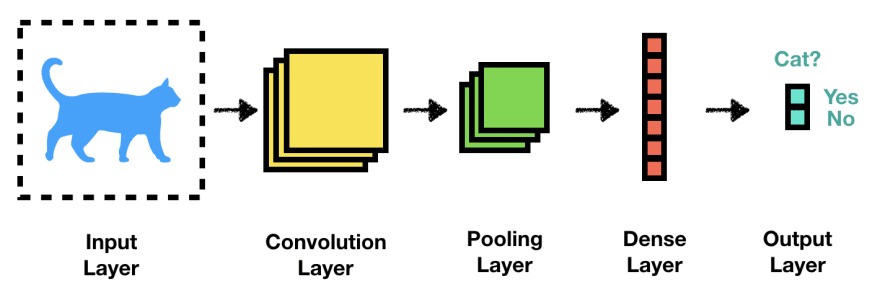
\includegraphics[width=0.45\textwidth]{pictures/cnn.png}
    \caption{Representation of the layered structure in a convolutional neural network.}
    \label{fig:cnn}
\end{figure}

\subsection{Evaluation of the classifiers}
% A critical evaluation of your two models.  
% How are you measuring their performance?  
% How did they do?  
% Which model gave the best results?  
% Include at least five predictions in the report (both good and bad).


Performance of the CNN is measured when the trained model is evaluated with the test samples. In Keras, there is a function called \verb|evaluate()| that outputs the test loss and test accuracy. The SVM accuracy was obtained by creating a function that cross-validates the predictions of the test-set with their real value. The common performance measure for the two models will therefore be the accuracy.

Figure \ref{fig:accSVM} and \ref{fig:accCNN} displays some samples from the classification process with SVM and CNN, respectively. Above each image, both the true label and the prediction is given. Looking at nine random predictions made by the models, which has an accuracy of about 80-90\%, at least one of the predictions should be a wrong classification. The prediction in the upper left corner of figure \ref{fig:accSVM} is an example of a faulty prediction. If we were to speculate, it might be that the dataset contains more lower-case \textit{t}'s rather than upper-cases (\textit{T}), and the opposite is true for an \textit{i}. On the other side, the image is very blurry, which might have been preventable by supplementing the training data with blurred copies of the original data. Another bad prediction can be seen by the prediction in the upper right and lower left corner of the CNN predictions in figure \ref{fig:accCNN}. The lower left "i" was predicted as a "l", which is understandable given that bottom of the next letter in the image will trick the CNN into thinking that these pixels are more likely connected.

\begin{figure}[H]
    \centering
    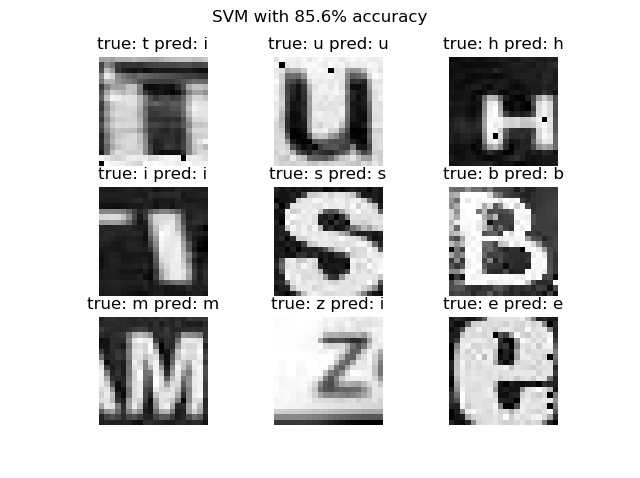
\includegraphics[width=0.45\textwidth]{pictures/accSVM.png}
    \caption{Samples from the classification process with SVM.}
    \label{fig:accSVM}
\end{figure}

\begin{figure}[H]
    \centering
    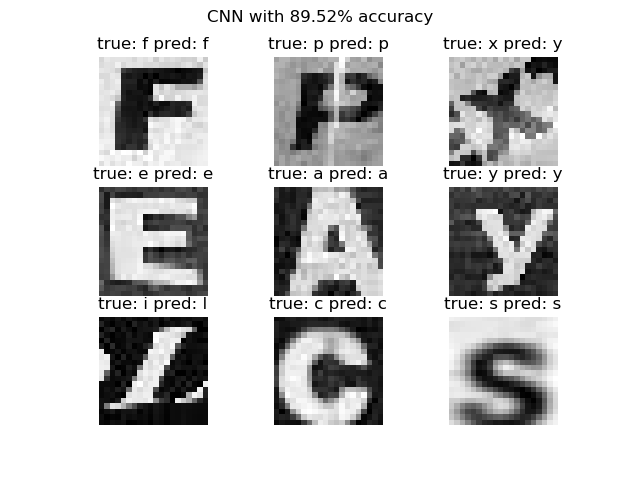
\includegraphics[width=0.45\textwidth]{pictures/accCNN.png}
    \caption{Samples from the classification process with CNN.}
    \label{fig:accCNN}
\end{figure}

As it can be seen from the samples above, both models achieved a good accuracy. However, the overall highest accuracy was as expected accomplished by CNN with \textasciitilde 89\%, as to \textasciitilde 85\% for the SVM.

\subsection{Alternative classifiers}
% Were there any additional models that you would have liked to try, but for some reason were notable to?  Explain.

It would be interesting to test the k-Nearest Neighbour (k-NN) algorithm for character classification. It would be fun to know the accuracy of such a straightforward and humble algorithm. The k-NN algorithm would probably work best if we performed some of the same pre-processing steps as for the SVM, such as converting to gray-scale (potentially binary) and extracting the HOG.

Another method we could have implemented for this project is ensemble methods, which use various learning algorithms to obtain a better prediction than the models would get individually. Aggregating a diverse set of models into one would make it more robust and able to handle new data much better. We could have, for instance, combined the result of both of our methods to produce a more favorable result. 




